%%%%%%%%%%%%%%%%%%%%%%%%%%%%%%%%%%%%%%%%%
% Diaz Essay
% LaTeX Template
% Version 2.0 (13/1/19)
%
% This template originates from:
% http://www.LaTeXTemplates.com
%
% Authors:
% Vel (vel@LaTeXTemplates.com)
% Nicolas Diaz (nsdiaz@uc.cl)
%
% License:
% CC BY-NC-SA 3.0 (http://creativecommons.org/licenses/by-nc-sa/3.0/)
%
%%%%%%%%%%%%%%%%%%%%%%%%%%%%%%%%%%%%%%%%%

%----------------------------------------------------------------------------------------
%	PACKAGES AND OTHER DOCUMENT CONFIGURATIONS
%----------------------------------------------------------------------------------------

\documentclass[11pt]{diazessay} % Font size (can be 10pt, 11pt or 12pt)
% -- Loading the code block package:
\usepackage{listings}
% -- Basic formatting
\usepackage[utf8]{inputenc}
\usepackage[english]{babel}
\usepackage{times}
\setlength{\parindent}{8pt}
\usepackage{indentfirst}
% -- Defining colors:
\usepackage[dvipsnames]{xcolor}
\definecolor{codegreen}{rgb}{0,0.6,0}
\definecolor{codegray}{rgb}{0.5,0.5,0.5}
\definecolor{codepurple}{rgb}{0.58,0,0.82}
\definecolor{backcolour}{rgb}{0.95,0.95,0.92}
% Definig a custom style:
\lstdefinestyle{mystyle}{
    backgroundcolor=\color{backcolour},
    commentstyle=\color{codepurple},
    keywordstyle=\color{NavyBlue},
    numberstyle=\tiny\color{codegray},
    stringstyle=\color{codepurple},
    basicstyle=\ttfamily\footnotesize\bfseries,
    breakatwhitespace=false,
    breaklines=true,
    captionpos=t,
    keepspaces=true,
    numbers=left,
    numbersep=5pt,
    showspaces=false,
    showstringspaces=false,
    showtabs=false,
    tabsize=2
}
% -- Setting up the custom style:
\lstset{
  style=mystyle,
  framexleftmargin=3.5mm,
  frame=shadowbox,
  rulesepcolor=\color{black},
  linewidth=0.6\linewidth,
  xleftmargin=12pt,
  aboveskip=12pt,
  belowskip=12pt
}

%----------------------------------------------------------------------------------------
%	TITLE SECTION
%----------------------------------------------------------------------------------------

\title{\textbf{Natural Language Processing} \\ {\Large\itshape With Tweets}} % Title and subtitle

\author{\textbf{Ruben Gonzalez, Mason Speck} \\ \textit{Texas State University}} % Author and institution

\date{\today} % Date, use \date{} for no date

%----------------------------------------------------------------------------------------

\begin{document}

\maketitle % Print the title section

%----------------------------------------------------------------------------------------
%	ABSTRACT AND KEYWORDS
%----------------------------------------------------------------------------------------

%\renewcommand{\abstractname}{Summary} % Uncomment to change the name of the abstract to something else

\begin{abstract}
This research aims to utilize natural language processing to produce a machine learning model capable of classifying posts from users of the social media website Twitter as pertaining, or not pertaining, to occurrences of natural disasters. Using a corpus of training and testing data provided by the company Figure Eight, four machine learning models were trained and optimized against already-classified posts from Twitter. After training the models, predictions were ran against a corpus of new, unclassified, and unseen Twitter posts and the accuracy of each of the models evaluated. The four models utilized were multinomial naive Bayes, random forest, logistic regression, and a multi-layer perceptron convolutional neural network (MLP). Of these models, the multinomial naive Bayes model performed the best, accurately classifying 80.21\% of previously unseen and unclassified Twitter posts.
\end{abstract}

\vspace{30pt} % Vertical whitespace between the abstract and first section

%----------------------------------------------------------------------------------------
%	ESSAY BODY
%----------------------------------------------------------------------------------------

\section*{Introduction}

Natural disasters cause significant harm and loss to individuals, communities, and infrastructure worldwide. It's crucial to obtain accurate and timely information about natural disasters, including their location, magnitude, and impact, to ensure an effective emergency response. Social media, particularly Twitter, has become an essential tool for people to communicate and disseminate information during a disaster. However, filtering relevant information from the vast amounts of data on Twitter during a natural disaster can be challenging.

Natural Language Processing (NLP) is a powerful tool in the field of machine learning that has been gaining increased attention in recent years. One application of NLP is the classification of Twitter posts as pertaining to natural disasters or not. This has become a particularly relevant issue as social media platforms like Twitter have become an important source of real-time information during disasters, both for individuals seeking help and for emergency response teams looking to coordinate relief efforts.

Our research project aims to use NLP to build a machine learning model that can accurately classify Twitter posts related to natural disasters. To achieve this, we used a corpus of training and testing data provided by Kaggle \cite{nlp-getting-started}, which contained already-classified posts from Twitter. We trained and optimized four different machine learning models, including multinomial naive Bayes, random forest, logistic regression, and a multi-layer perceptron convolutional neural network (MLP).

After training the models, we evaluated their accuracy against a corpus of new, unclassified, and unseen Twitter posts. Our results showed that the multinomial naive Bayes model performed the best, accurately classifying 80.21 of previously unseen and unclassified Twitter posts. This high accuracy rate is particularly noteworthy considering the noisy and unstructured nature of Twitter data.

Our work is part of a Kaggle competition, where we are competing against other teams to develop the most accurate model for classifying disaster-related tweets. This competition provides an opportunity to explore the potential of NLP and machine learning in addressing real-world problems, and we are excited to be contributing to this field of research.
%------------------------------------------------

\section*{Methodology}
\subsection{Imports}

When working on Natural Language Processing (NLP) projects, it is important to import the necessary libraries to process text data and build machine learning models. Let's go through the libraries imported in the code snippet above and their functions:

\verb|Pandas|: Pandas is a library that provides data structures and functions to manipulate numerical tables and time-series data. In this code, it is used to read in the dataset containing text data.

\verb|Matplotlib|: Matplotlib is a plotting library that allows for the creation of various types of plots, including line, bar, scatter, and histogram plots. In this code, it is used to create visualizations of the performance of different models.

\verb|Seaborn|: Seaborn is a visualization library that provides a high-level interface for creating informative and attractive statistical graphics. In this code, it is used to create visualizations of the performance of different models.

\verb|sklearn.metrics|: This library provides a suite of functions for evaluating the performance of machine learning models. In this code, we use the ROC curve display, confusion matrix, and F1 score to evaluate model performance.

\verb|NLTK| (Natural Language Toolkit): NLTK is a library for working with human language data, including tokenization, stemming, and lemmatization. In this code, we use the NLTK library for tokenization, lemmatization, and stop word removal.

\verb|sklearn.model_selection|: This library provides functions for splitting data into training and testing sets, as well as cross-validation. In this code, we use it to split our data into training and testing sets.

\verb|sklearn.feature_extraction.text|: This library provides tools for feature extraction from text data. In this code, we use the TfidfVectorizer to convert our text data into numerical features that can be used in machine learning models.

\verb|sklearn.naive_bayes|: This library provides implementations of Naive Bayes algorithms for classification. In this code, we use the Multinomial Naive Bayes algorithm for text classification.

\verb|sklearn.ensemble:| This library provides implementations of ensemble algorithms, including Random Forest, which we use for text classification in this code.

\verb|sklearn.linear_model|: This library provides implementations of various linear models, including logistic regression, which we use for text classification in this code.

\verb|sklearn.neural_network|: This library provides an implementation of a multi-layer perceptron (MLP) neural network, which we use for text classification in this code.

The libraries imported in this code are necessary for processing text data, building machine learning models, and evaluating their performance. By importing these libraries, we have access to a variety of functions and tools that make it easier to work with text data and build effective models for text classification. Let's move on and look at the data we are importing.

\subsection{Quick look at our data}

 The dataset consists of three CSV files: train.csv, test.csv, and sample\textunderscore submission.csv. The train.csv file contains the labeled data used to train a machine learning model to predict whether a tweet is about a real disaster or not, denoted by a binary target variable. The test.csv file contains unlabeled data that will be used to evaluate the performance of the trained model. Finally, the sample \textunderscore submission.csv file is provided as a template for submitting to Kaggle.

Next, let's take a closer look at the train.csv file. The file contains the following columns:
\begin{itemize}
\item id: a unique identifier for each tweet
\item text: the text of the tweet
\item location: the location the tweet was sent from (may be blank)
\item keyword: a particular keyword from the tweet (may be blank)
\item target: in train.csv only, this denotes whether a tweet is about a real disaster (1) or not (0)
\end{itemize}

It's important to note that the keyword and location columns may contain missing values, denoted by NaN. Additionally, the text column contains text data, while the target variable is a binary indicator. To load the train.csv and test.csv files into Pandas dataframes, the following code can be used:

\begin{lstlisting}[language=Python]
import pandas as pd

train_df = pd.read_csv("data/train.csv")
test_df = pd.read_csv("data/test.csv")
train_df.head()
\end{lstlisting}


The head() method is then used to display the first five rows of the train \textunderscore df dataframe. Once the data is loaded, the next step would be to explore and clean the data as needed. This may involve removing missing values, handling text data by removing stop words, tokenizing, stemming, and other techniques to prepare the data for analysis. Let's look at prepossessing.

\subsection{Preprocess data}

Preprocessing is an essential step in machine learning tasks that involves transforming the raw data into a format that can be easily understood by the machine learning models. Preprocessing helps to improve the quality of data, reduce noise, and make it easier for the models to understand the data.

First, we remove unnecessary columns such as 'id', 'keyword', and 'location' from both the train and test datasets. These columns do not provide any useful information for the task at hand, which is classifying whether a tweet refers to a real disaster or not. Next, we define three preprocessing functions that will be used to preprocess the 'text' column in both the train and test datasets. The first function is remove \textunderscore stopwords, which removes common words that do not add any useful information to the dataset. We use the stopwords library from the Natural Language Toolkit (NLTK) to obtain a set of commonly used English stopwords. We then use list comprehension to remove the stopwords from the text column, and finally, join the remaining words to form a new string.

The second function is apply \textunderscore stemming which reduces words to their root form by removing suffixes. We use the Porter Stemmer algorithm, which is also implemented in the NLTK library. The algorithm works by applying a set of rules to remove the suffixes and produce the root form of the word. The third function is apply \textunderscore lemmatization, which is similar to stemming but produces a meaningful root form of the word, known as a lemma. The lemmatization algorithm considers the part of speech of the word and produces a meaningful root form. We use the WordNet Lemmatizer algorithm, which is also implemented in the NLTK library.

Finally, we apply the three preprocessing functions to the 'text' column in both the train and test datasets. We use the 'apply' method in pandas to apply the functions to each row in the 'text' column. The 'lambda' function is used to apply each function sequentially. Preprocessing has several benefits. Firstly, it helps to reduce the dimensionality of the dataset, which makes it easier for the models to process the data. Secondly, it helps to remove noise from the data, such as stop words and suffixes, which can lead to more accurate predictions. Lastly, it helps to improve the interpretability of the data by reducing the complexity of the language used in the tweets.

\subsection{Defining feature vector and splitting data into sets}

The feature vector is a representation of the text data in a numerical format that the machine learning algorithm can understand. In this code, the \verb|TfidfVectorizer| from scikit-learn library is used to convert the text into a numerical format that can be used for training the model. The \verb|TfidfVectorizer| takes the text as input and outputs a matrix where each row represents a document and each column represents a term from the text. The values in the matrix represent the importance of each term in the document. The target variable in this code is the "target" column from the \verb|train_df_dataframe|. This column represents whether a tweet is referring to a real disaster or not (1 for real disaster and 0 for not a real disaster).

After defining the feature vector and target variable, the next step is to split the data into a training set and a testing set. This is done to evaluate the performance of the model on unseen data. In this code, the \verb|train_test_split| method from scikit-learn library is used to randomly split the data into a training set and a testing set. The \verb|test_size| parameter is set to 0.2, which means that 20\% of the data will be used for testing, while 80\% will be used for training. The \verb|random_state| parameter is set to 42 to ensure reproducibility of the results.

The \verb|train_test_split| method returns four arrays: \verb|X_train|, \verb|X_test|, \verb|y_train|, and \verb|y_test|. \verb|X_train| and \verb|y_train| are used for training the model, while \verb|X_test| and \verb|y_test| are used for evaluating the performance of the model on unseen data.

\subsection{Train a Multinomial Naive Bayes, Random Forest, Logistic Regression, and MLP model}

First step in the code initializes a dictionary to store the results of each model that is trained and tested. This dictionary will be used to compare the performance of each model. Four different models are trained and tested on the data.

The first model is the Multinomial Naive Bayes model. In this model, the alpha hyperparameter is set to 0.6. This hyperparameter controls the smoothing of the probabilities in the model. A higher alpha value leads to more smoothing and can prevent overfitting. The fit method is called on the training data to train the model. Then, the predict method is called on the test data to make predictions. The \verb|f1_score| method is used to compute the F1 score for the model's predictions. The F1 score is a measure of the model's accuracy that takes both precision and recall into account. Finally, the \verb|classification_report| function is called to print out the precision, recall, and F1 score for each class, as well as the overall accuracy of the model. The results of this model are saved in the dictionary with the key "Multinomial Naive Bayes".

The second model is the Random Forest model. In this model, the \verb|n_estimators| hyperparameter is set to 200. This hyperparameter controls the number of decision trees that are created in the random forest. The \verb|random_state| hyperparameter is set to 42 to ensure reproducibility of the results. The same process as the Multinomial Naive Bayes model is followed to train and test this model. The results of this model are saved in the dictionary with the key "Random Forest".

The third model is the Logistic Regression model. This model does not have any hyperparameters specified. The same process as the previous models is followed to train and test this model. The results of this model are saved in the dictionary with the key "Logistic Regression".

The fourth and final model is the Convolutional Neural Network (CNN) model. This model is defined using the MLPClassifier class. The \verb|hidden_layer_sizes| hyperparameter is set to (10,), which means that the model has one hidden layer with 10 neurons. The \verb|max_iter| hyperparameter is set to 100, which controls the maximum number of iterations that the solver will run. The alpha hyperparameter is set to 1e-4, which controls the L2 regularization parameter. The solver hyperparameter is set to "adam", which is an optimization algorithm that is commonly used for deep learning. The verbose hyperparameter is set to False, which means that no output will be printed during training. The tol hyperparameter is set to 1e-4, which controls the tolerance for the stopping criterion. The \verb|random_state| hyperparameter is set to 1 to ensure reproducibility of the results. Finally, the \verb|learning_rate_init| hyperparameter is set to 0.1, which controls the learning rate for the solver. The same process as the previous models is followed to train and test this model. The results of this model are saved in the dictionary with the key "MLP".

After all the models have been trained and tested, the model with the highest F1 score is determined using the max function on the results dictionary with a lambda function that selects the F1 score for each model. The best model is printed along with its F1 score and confusion matrix.

\subsection{Visualize data using ROC curves, confusion matrices and SNS heatmaps}

The code creates a 4 x 2 grid of plots, with each plot showing the performance evaluation of a different machine learning algorithm. The performance evaluation is done using two techniques: ROC curves and confusion matrices. ROC (Receiver Operating Characteristic) curves are a common technique used to evaluate the performance of binary classification models. The ROC curve is a graphical representation of the trade-off between the true positive rate (sensitivity) and the false positive rate (1 - specificity) for different classification thresholds. In the code above, ROC curves are plotted for each of the four machine learning algorithms using the \verb|RocCurveDisplay.from_estimator()| function. The ROC curves show how well the models can distinguish between the positive and negative classes, i.e., how well they can predict if a tweet is related to a natural disaster or not. A good classifier would have a ROC curve that closely follows the top-left corner of the plot, indicating high true positive rate and low false positive rate.

Confusion matrices are another way to evaluate the performance of a classification model. A confusion matrix is a table that shows the number of true positives (TP), true negatives (TN), false positives (FP), and false negatives (FN) for a binary classification problem. In the code above, confusion matrices are plotted using the \verb|confusion_matrix()| function from the scikit-learn library and the \verb|sns.heatmap()| function from the Seaborn library. The confusion matrices show the actual versus predicted class labels for the test set. The diagonal elements of the matrix represent the correct predictions, while the off-diagonal elements represent the incorrect predictions.

The heatmap function from the Seaborn library is used to plot the confusion matrix in a visually appealing way, with the color intensity indicating the number of correct or incorrect predictions. The \verb|annot=True| parameter in the \verb|sns.heatmap()| function is used to add the actual number of observations to the heatmap plot. This helps to get a better understanding of the model's performance and identify which classes the model is misclassifying.

\subsection{Predictions on test data}

The `model.predict()` function is used to predict the label of a given tweet. The function takes a set of input features and predicts the corresponding output class. The input features are the tweet texts, which are passed to the `vectorizer.transform()` method. The `vectorizer` object is a pre-trained model that converts the input text into a numerical vector that can be used as input to the machine learning model.

The transformed input data is then passed to the `model.predict()` method, which uses the trained model to predict the output class. The `model` object is initialized based on the best model selected from the training phase. If the best model is `Multinomial Naive Bayes`, then the `model` object is set to `nb`, which is the trained Naive Bayes model. Similarly, if the best model is `Random Forest`, then the `model` object is set to `rf`, which is the trained Random Forest model, and so on.

Once the `model.predict()` function is called, the model uses the input features to generate a prediction. The output of the `model.predict()` function is an array of predicted labels, where each label corresponds to a given tweet. The predicted labels are stored in the `predictions` variable. It is important to note that the `model.predict()` function relies on the accuracy and robustness of the machine learning model. A good machine learning model should have a high accuracy and be able to generalize well to new data. Additionally, the input features should be relevant to the task at hand and have a strong correlation with the output label. After running the models and gathering f1-scores, `Multinomial Naive Bayes` out-performed and was selected as the model to be used for prediction.


\section{Results}

% Results: use plots and tables to format your results. And also, add necessary description words to explain the results.

After fine-tuning the parameters of each of the four models fitted against the training data, predictions were ran against previously unseen and unclassified Twitter posts. All of the models were, ostensibly, similarly accurate, with the accuracy of the models ranging approximately 4\% between the most and least-accurate models. The accuracy of the models breaks down as follows:

\begin{center}
\begin{tabular}{ |c|c| }
  Model & Accuracy\\
  \hline
  Multinomial Naive Bayes & 80.21\%\\
  Random Forest & 78.92\%\\
  Logistic Regression & 79.14\%\\
  MLP & 76.21\%\\
\end{tabular}
\end{center}

Taking into consideration that there have been, on average, 200 billion posts made on Twitter every year since 2016, any percentage of difference in accuracy is significant, possibly measuring in millions of correct or incorrect classification results.

Considering the dangers posed by natural disasters, and the potential for significantly different classification results from each model, it became important to understand how each model performed beyond a single accuracy metric. To gain insight into the characteristics of each model's performance, we generated a number of aides:
\begin{enumerate}
  \item Receiver operating characteristic curves that plot a model's true positive rate against its false positive rate.
  \item Heatmaps of a model's confusion matrix, counting and visualizing the occurrence of true positive, true negative, false positive, and false negative results.
  \item Classification reports detailing a model's most important classification metrics
\end{enumerate}

% \bigskip\bigskip

% \begin{center}

\subsection{Multinomial Naive Bayes}

Multinomial naive Bayes (MNB) is a probabilistic classification algorithm. In our research, MNB was the most accurate of the four models, with a weighted average accuracy of 80.21\%. As seen in the figures below, the MNB model's receiver operating characteristic (ROC) curve was steady, with an area-under-curve score of approximately 85\%. The MNB model classified the highest amount of true positive results, the third-highest amount of true negative results, the second-highest amount of false positive results, and the least false negative results. The MNB model's values will be used as the baseline for comparisons against other models explored below.

\begin{minipage}[t]{.45\linewidth}
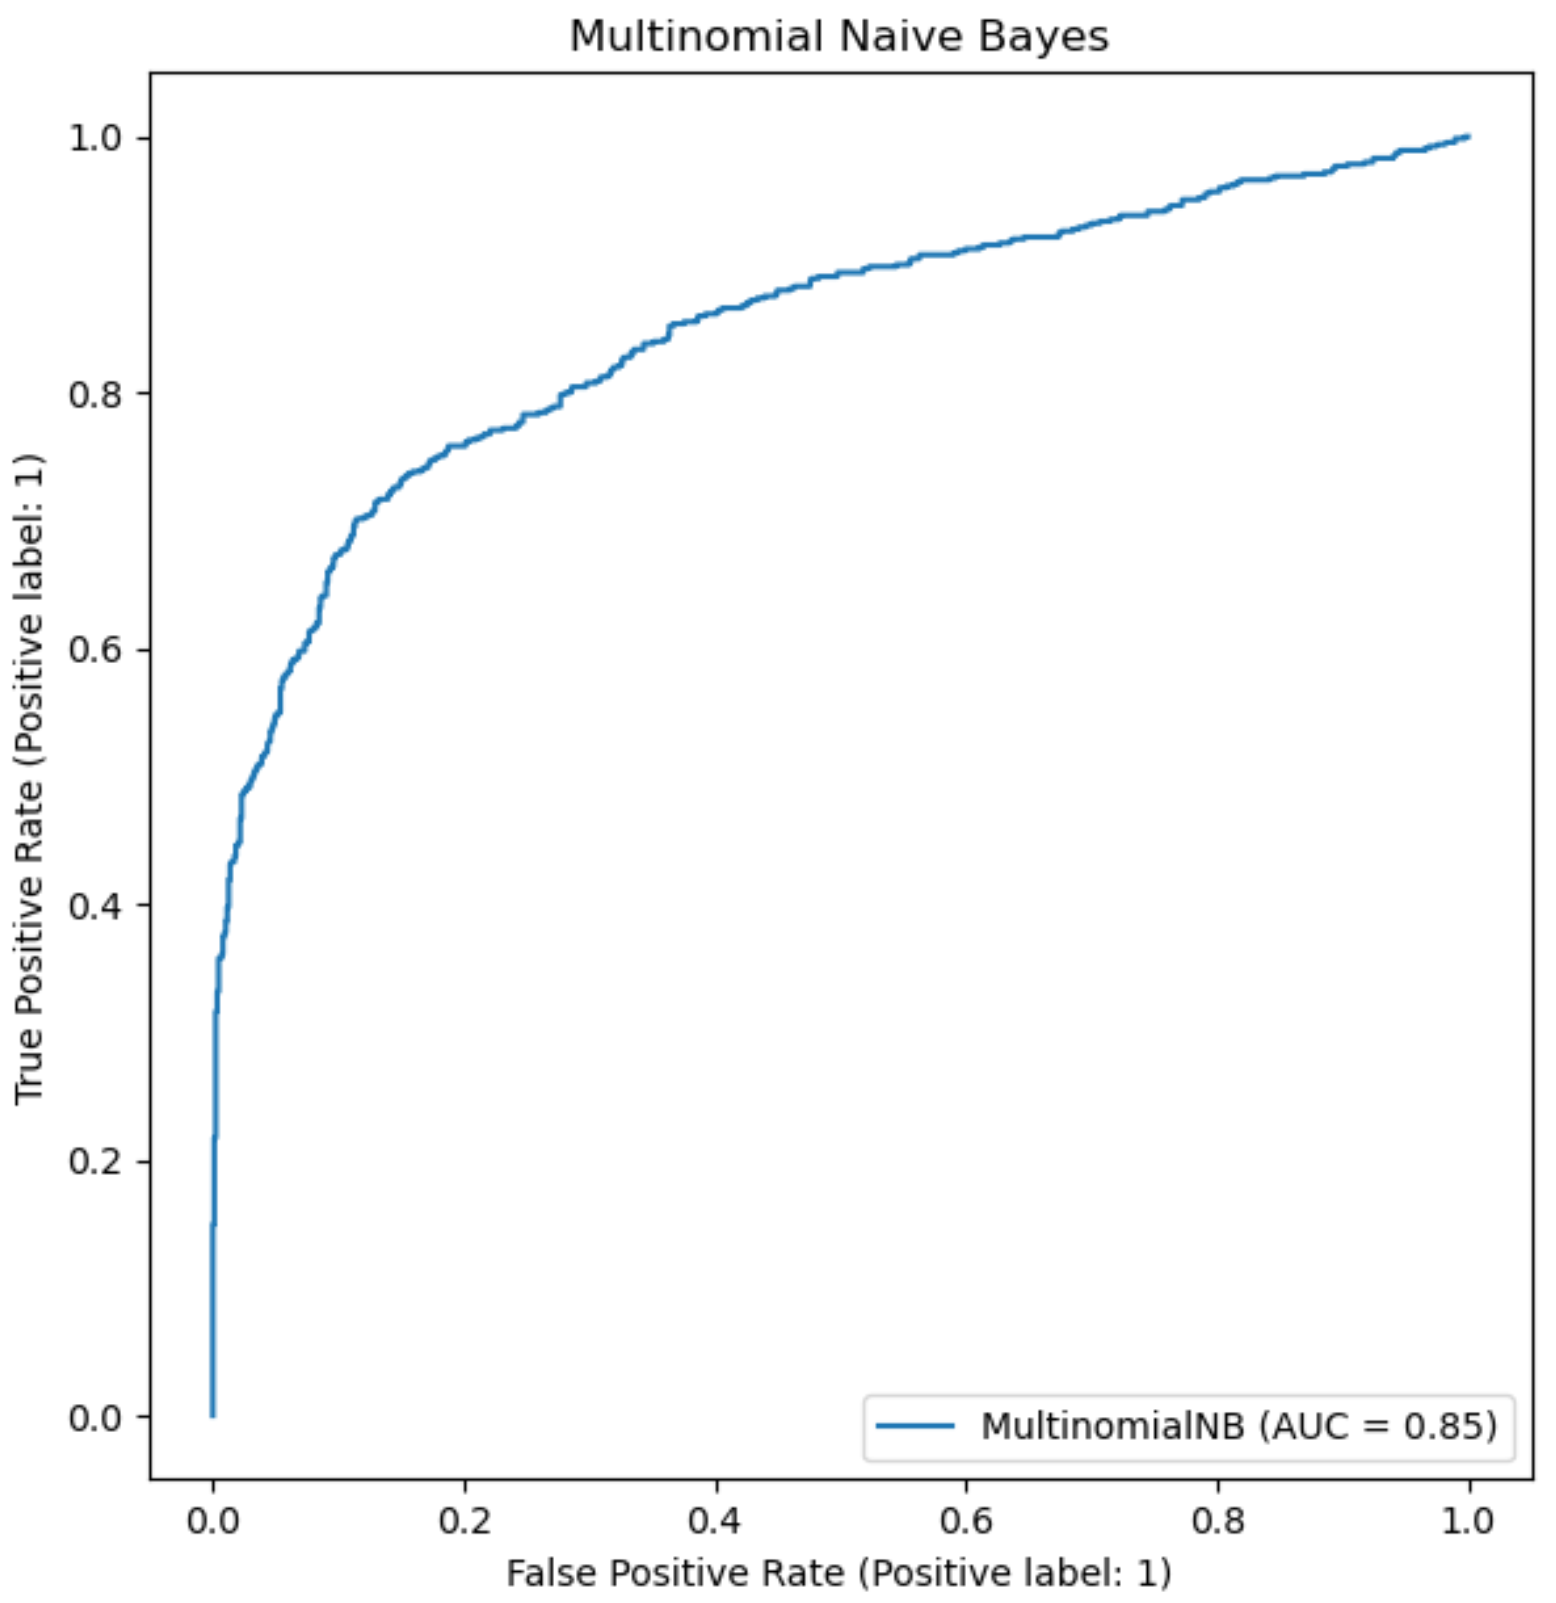
\includegraphics[width=\linewidth]{images/mnb_plot.png}
\end{minipage}\hfill
\begin{minipage}[b]{.45\linewidth}
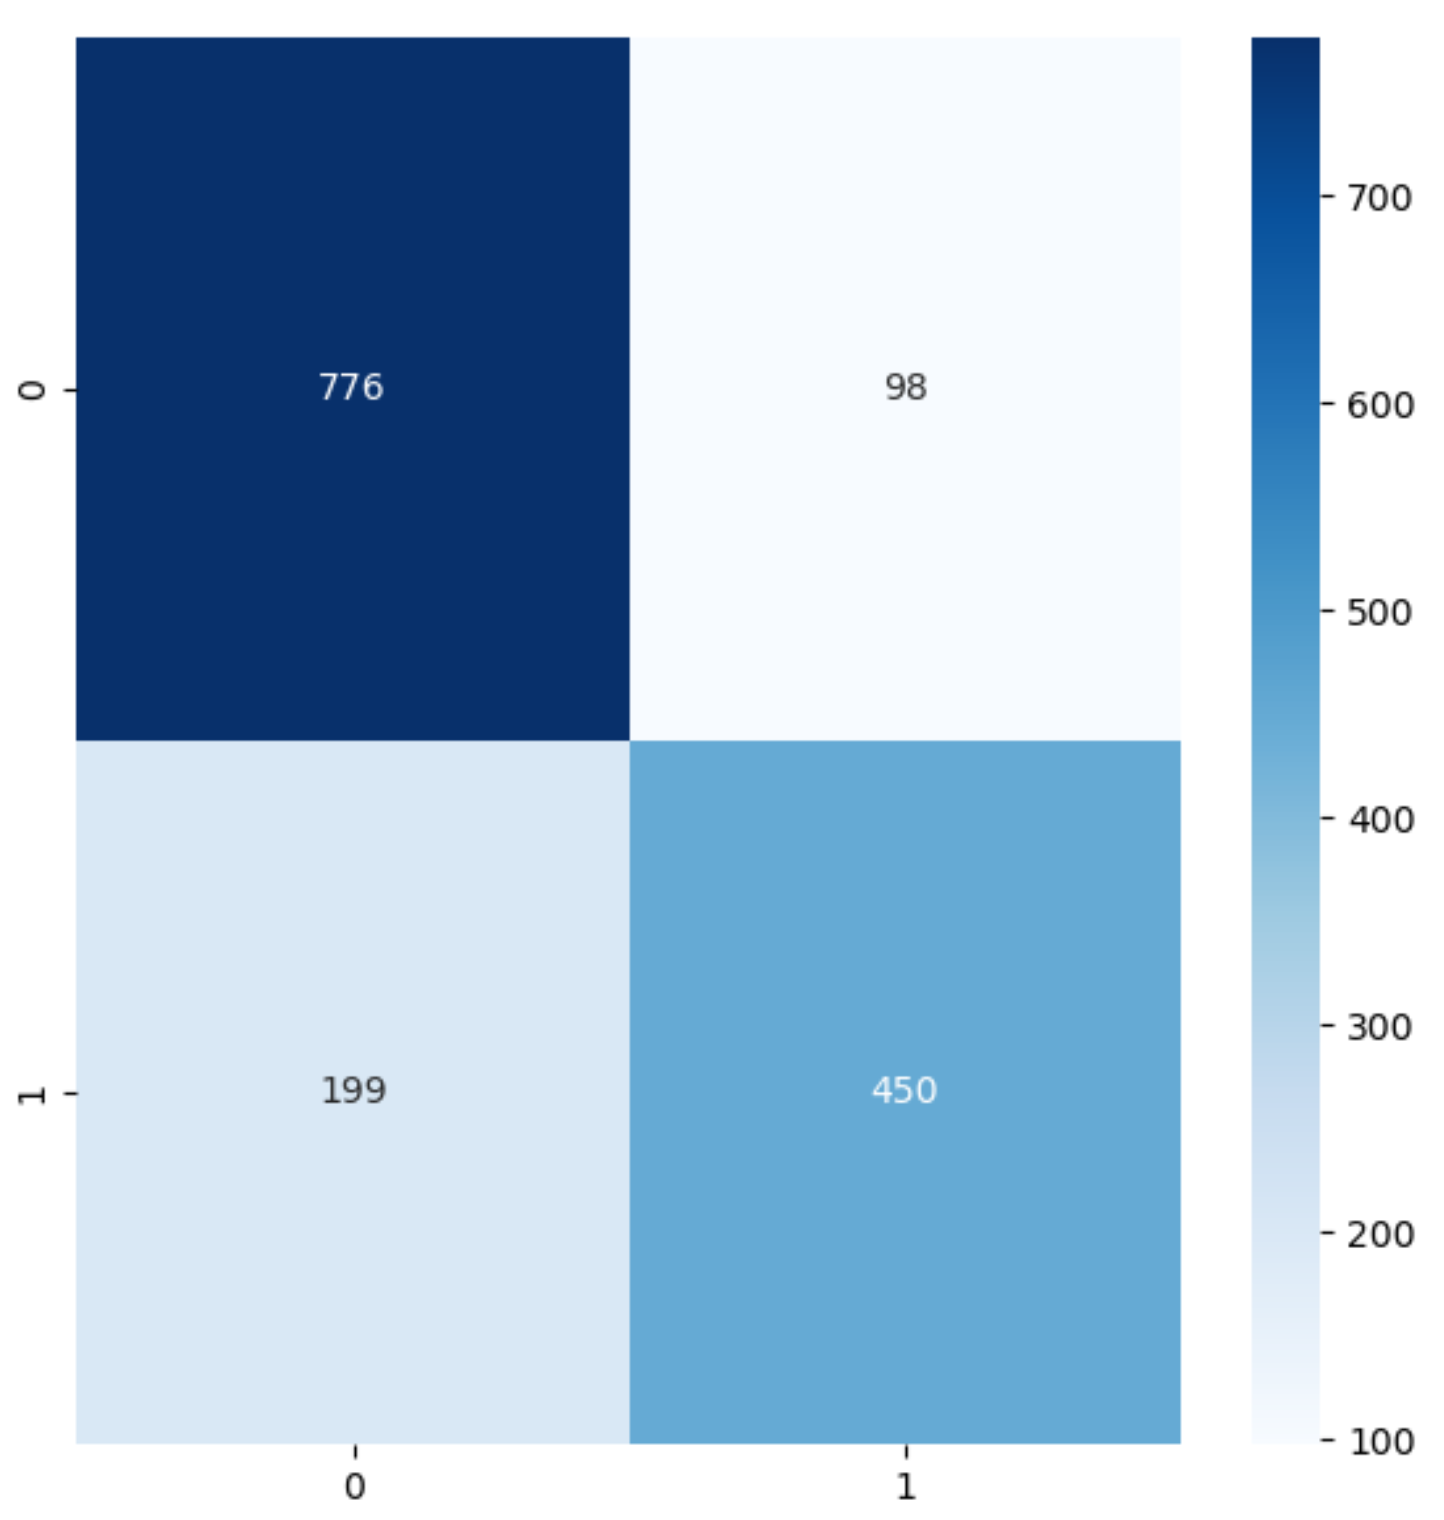
\includegraphics[width=\linewidth]{images/mnb_heatmap.png}
\end{minipage}\hfill

\subsection{Random Forest}

Random forest is a ensemble method useful for classification and regression. Random forest was the third-most accurate of the models we utilized, with a weighted average accuracy of 78.92\%. As with the MNB model, the random forest model's area-under-curve score was also approximately 85\%. Relative to MNB, the random forest model classified 90.23\% true positive results, 103.87\% true negative results, 69.39\% false positive results, and 122.11\% false negative results.

\begin{minipage}[t]{.45\linewidth}
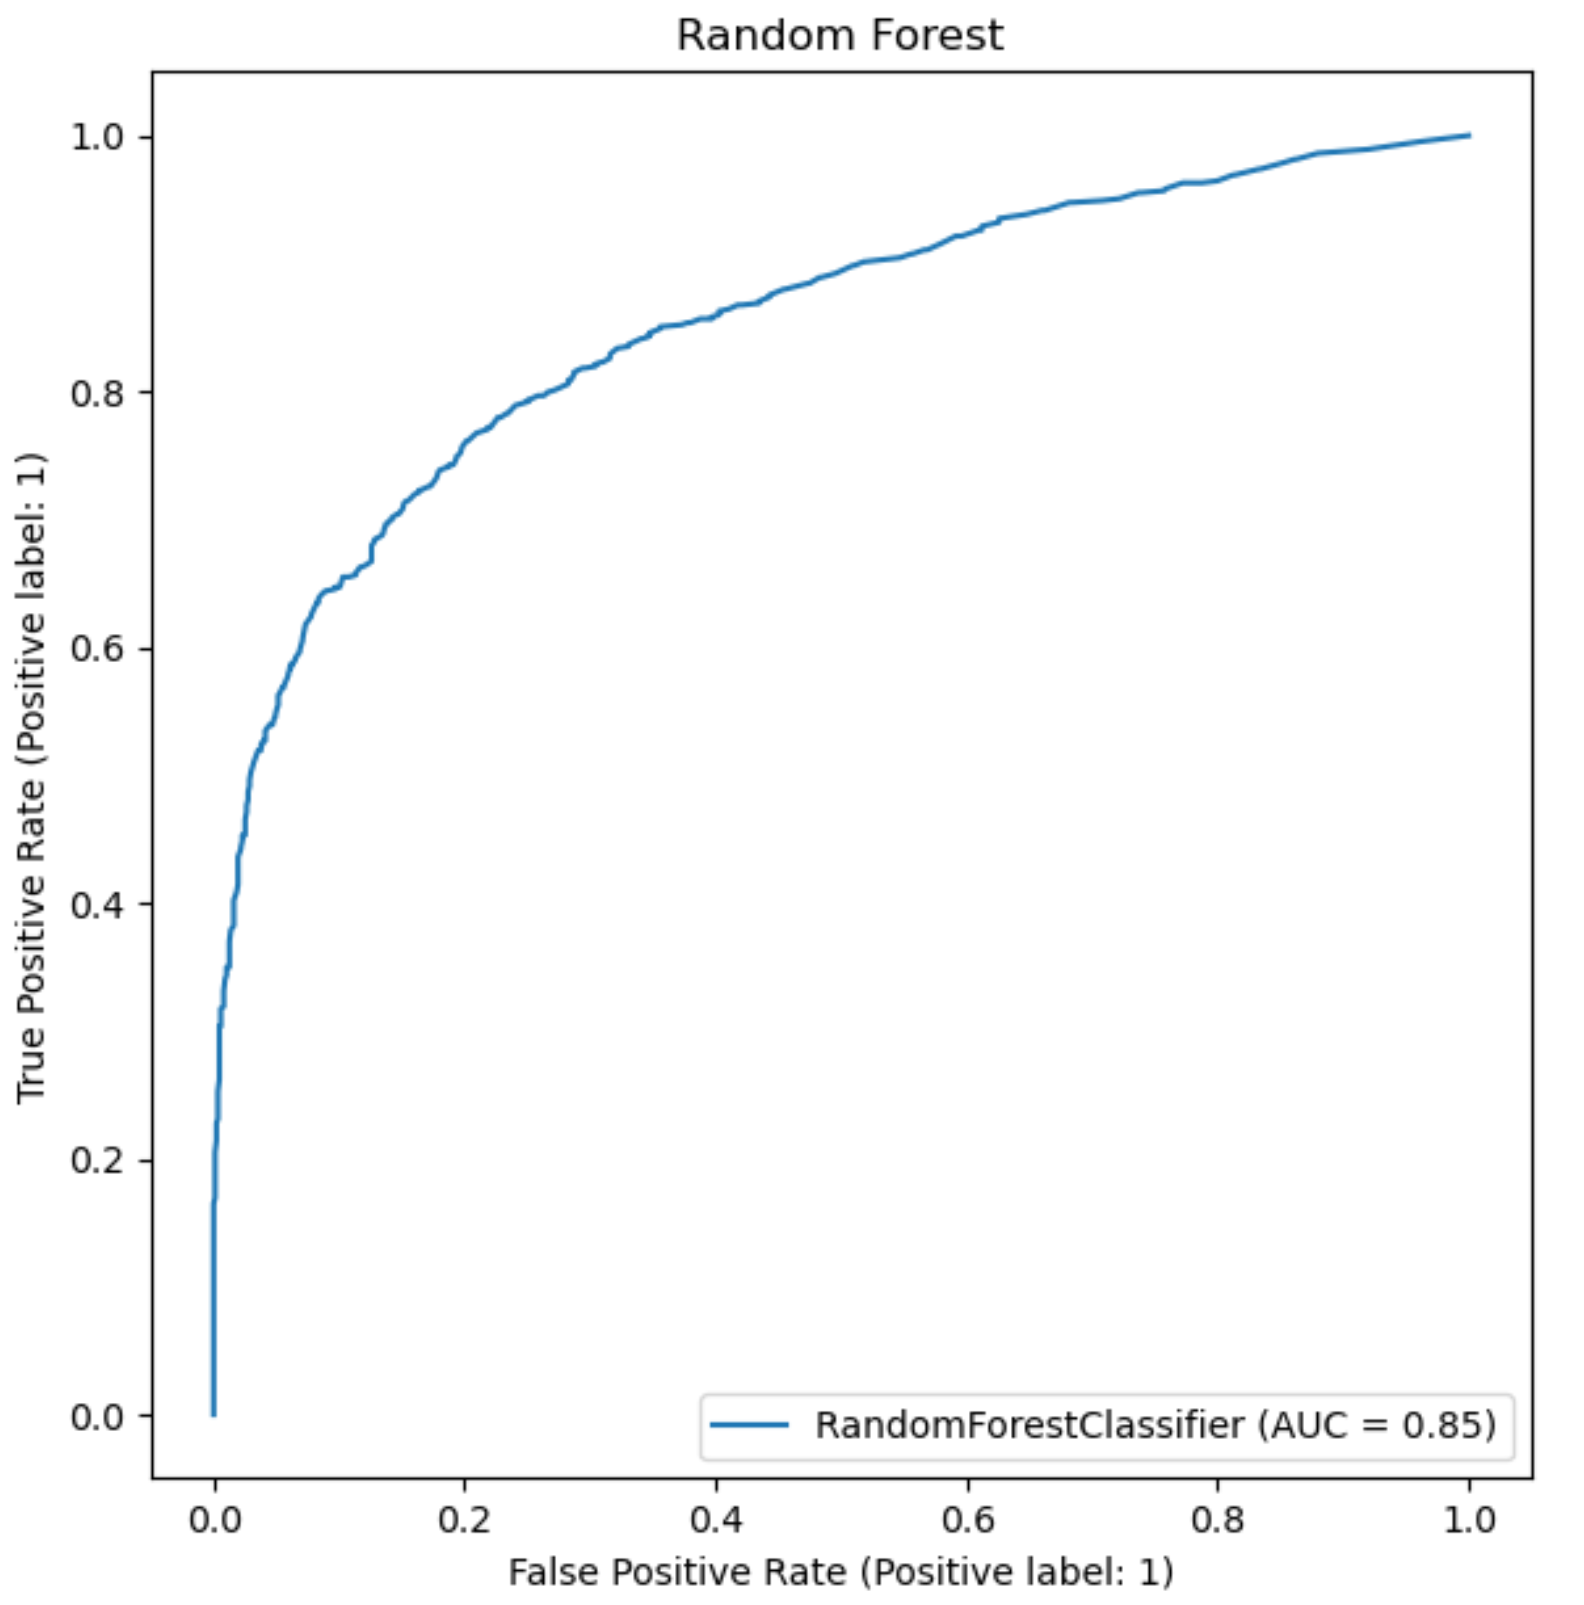
\includegraphics[width=\linewidth]{images/rf_plot.png}
\end{minipage}\hfill
\begin{minipage}[b]{.45\linewidth}
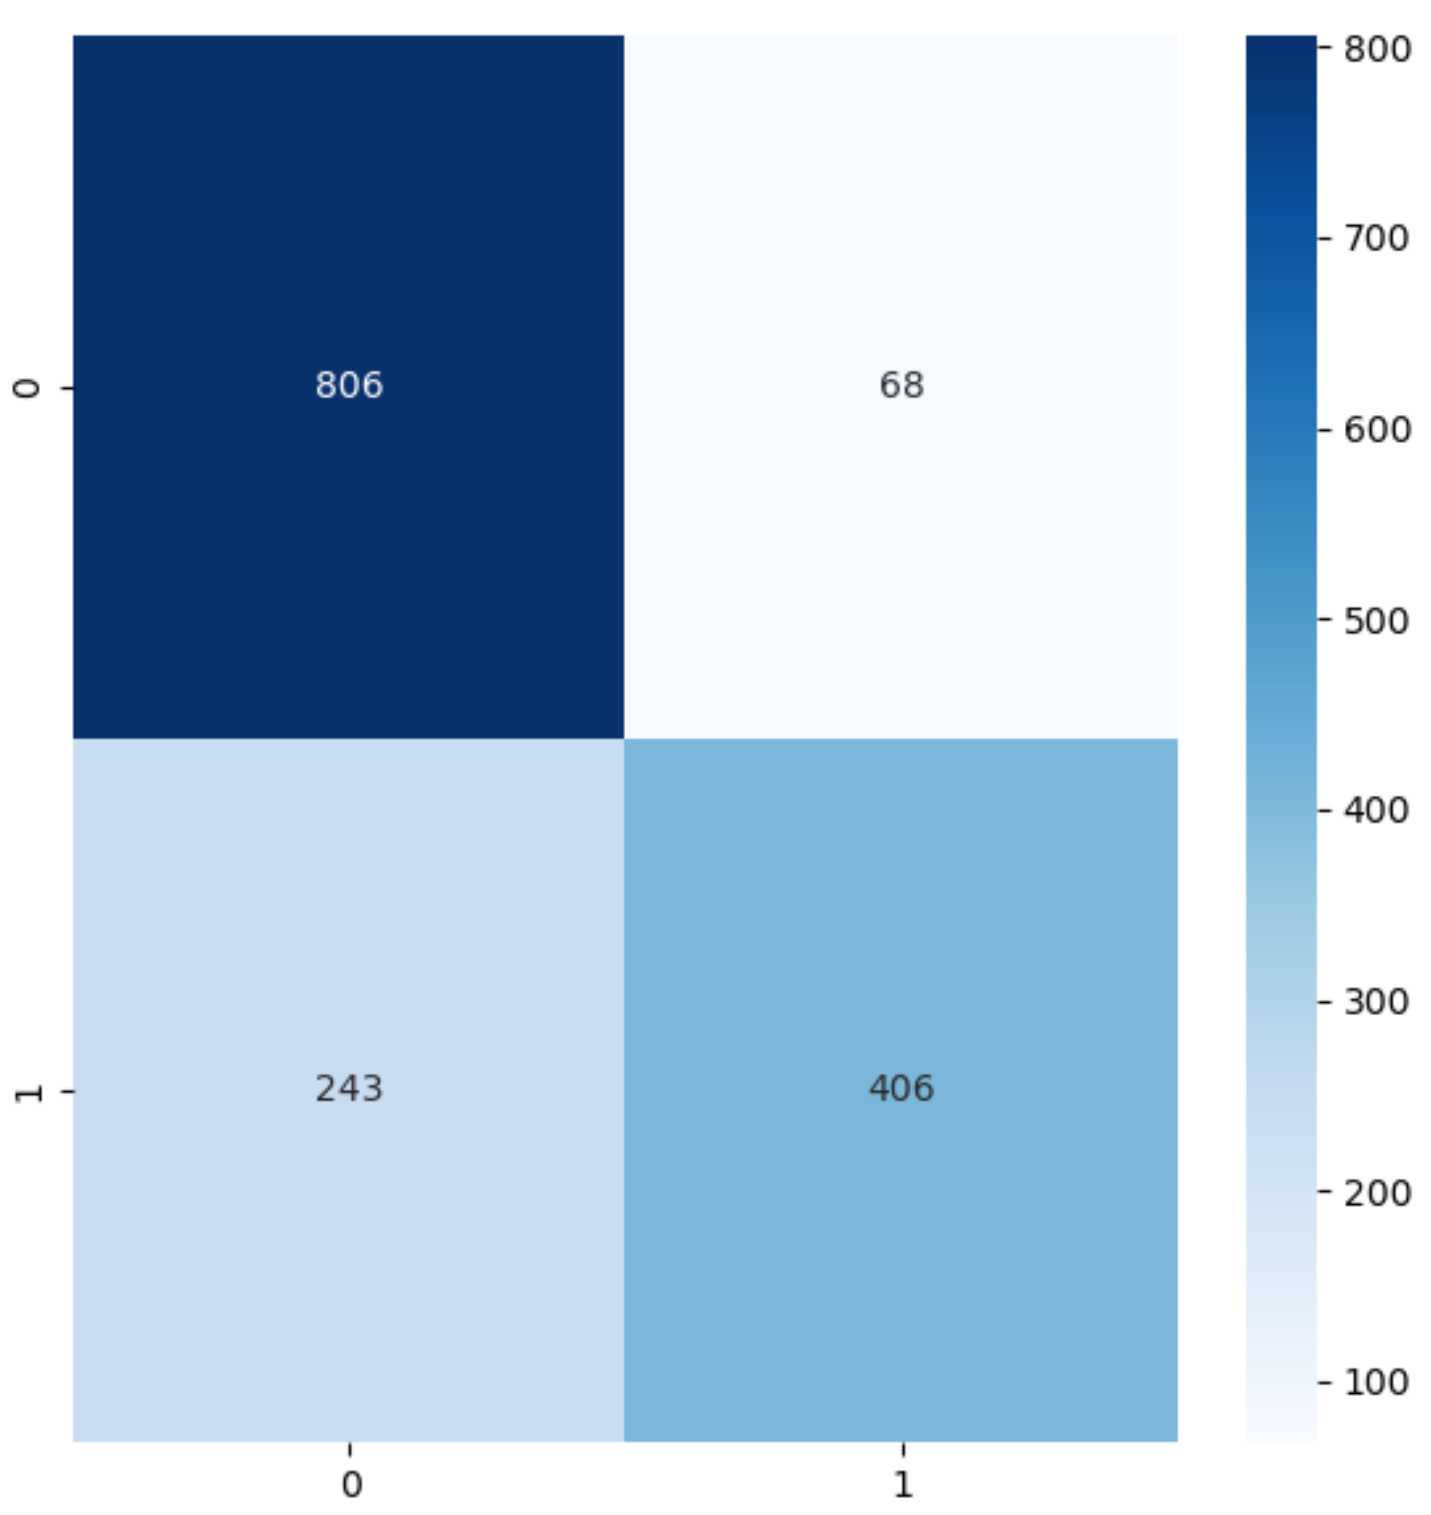
\includegraphics[width=\linewidth]{images/rf_heatmap.png}
\end{minipage}\hfill

\subsection{Logistic Regression}

Logistic regression is a regressor model that models the probabilities of linear combinations of independent variables. Logistic regression was the second-most accurate of the models in our research, with a weighted average accuracy of 79.14\%. The area-under-curve score for the logistic regression model's ROC plot was approximately 86\%. Relative to MNB, the logistic regression model classified 93.56\% true positive results, 102.10\% true negative results, 83.67\% false positive results, and 114.57\% false negative results.

\begin{minipage}[t]{.45\linewidth}
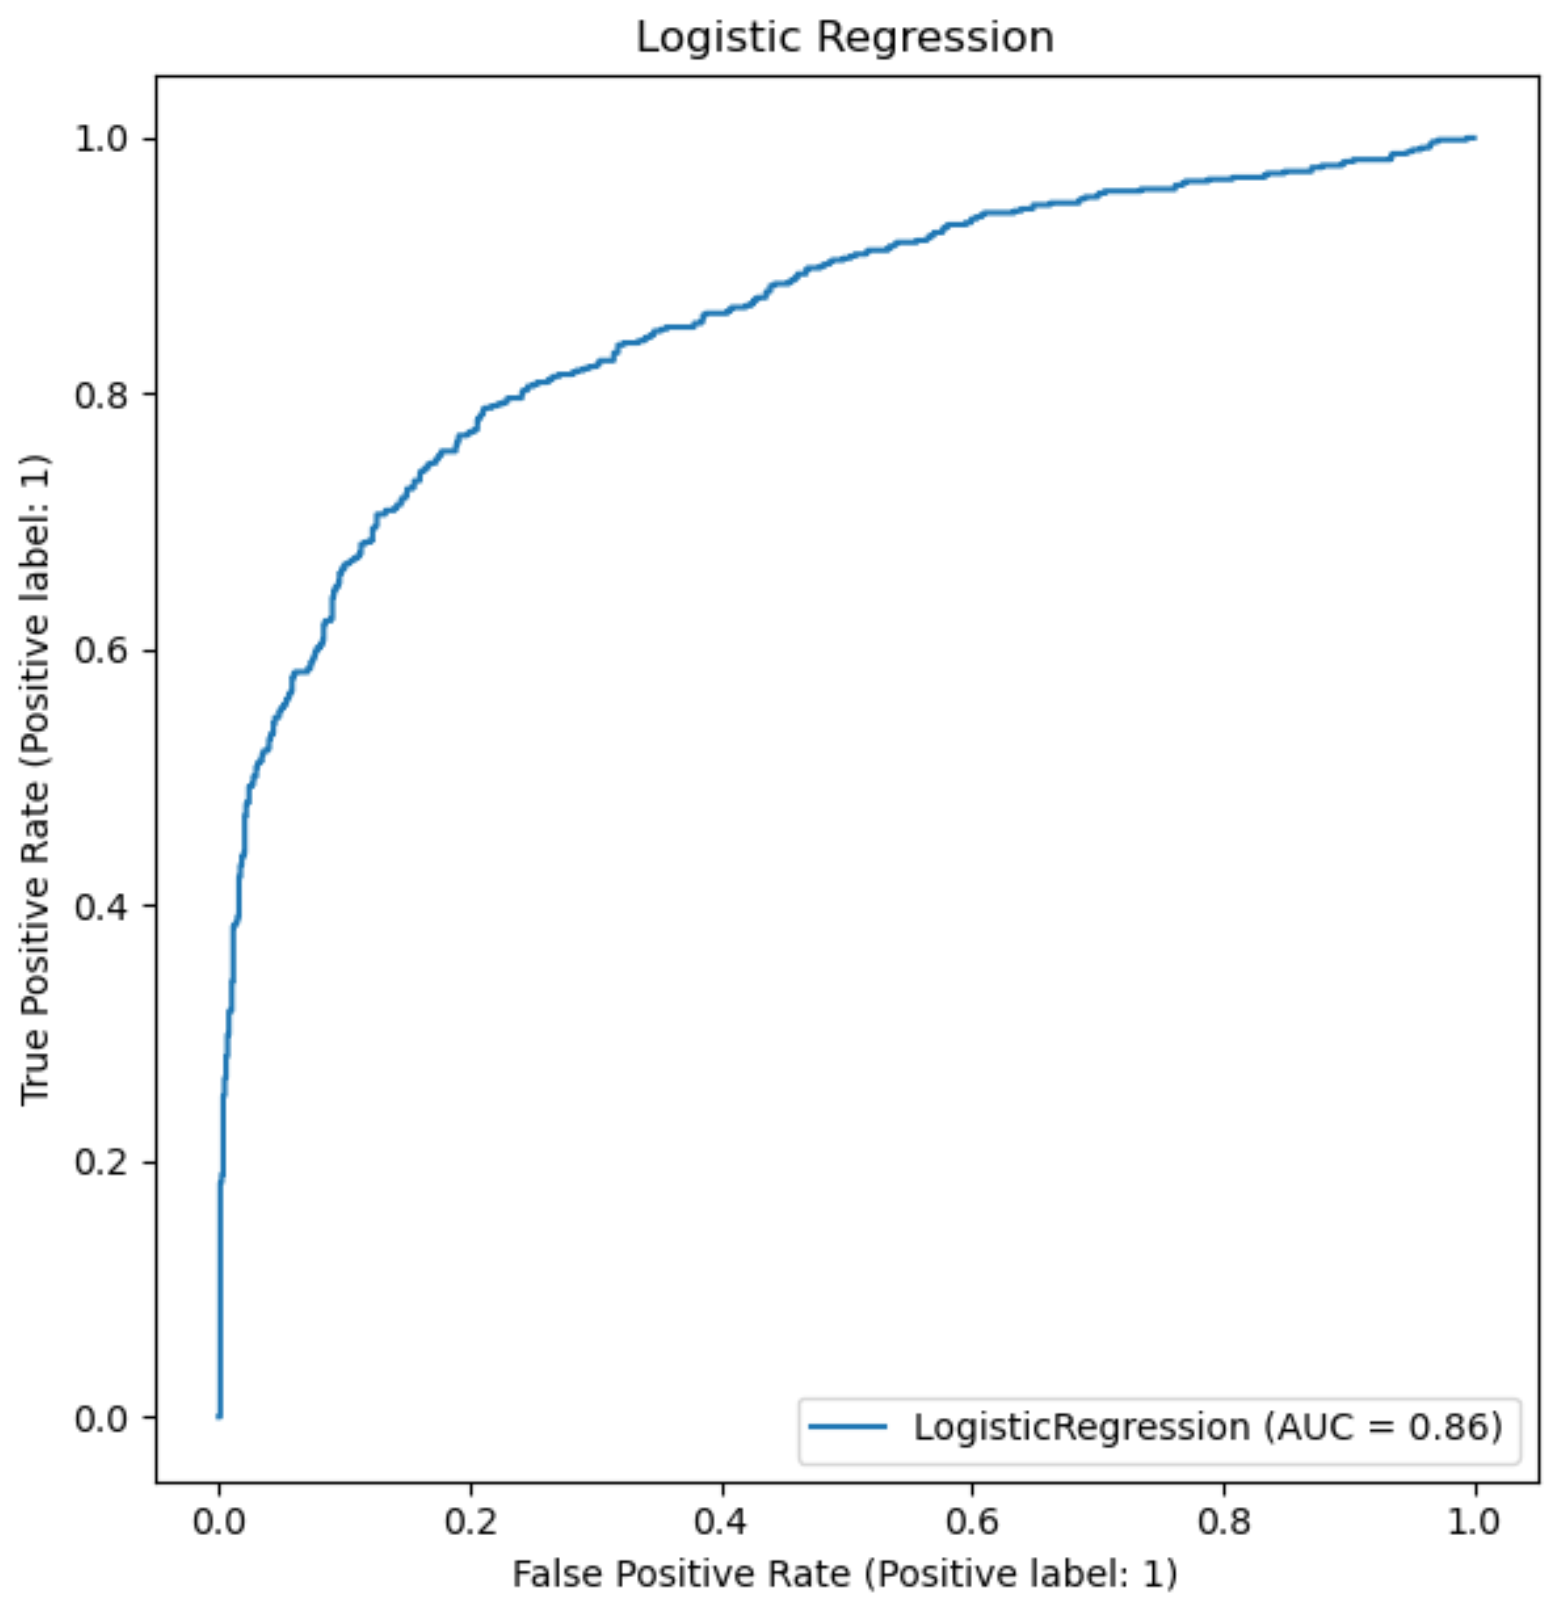
\includegraphics[width=\linewidth]{images/lr_plot.png}
\end{minipage}\hfill
\begin{minipage}[b]{.45\linewidth}
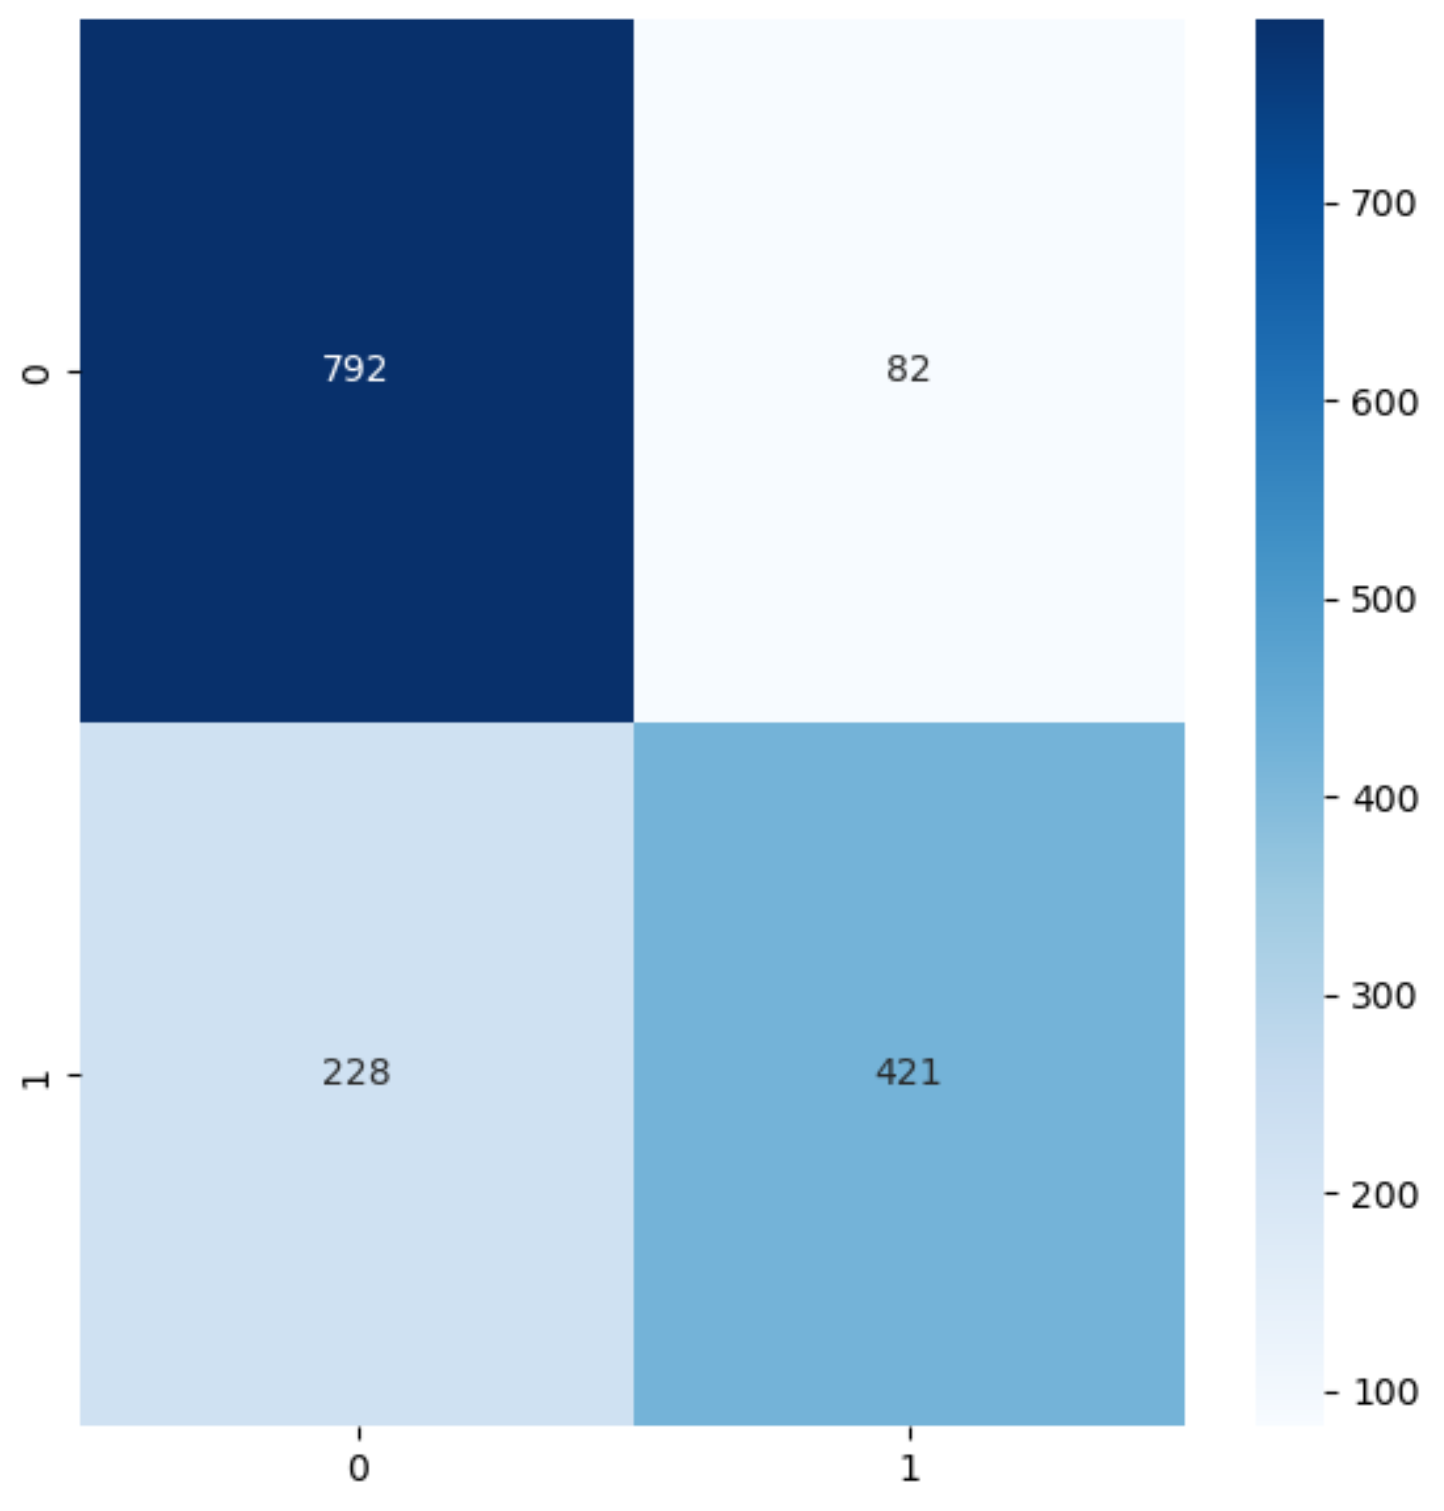
\includegraphics[width=\linewidth]{images/lr_heatmap.png}
\end{minipage}\hfill

\subsection{MLP}

The final model we used in our research was a multi-layer perceptron convolutional neural network (MLP). Compared to the other three models, the MLP model had the lowest weighted average accuracy score of 76.21\%. Relative to MNB, the MLP model classified 94.89\% true positive results, 95.10\% true negative results, 138.78\% false positive results, and 111.56\% false negative results.

\begin{minipage}[t]{.45\linewidth}
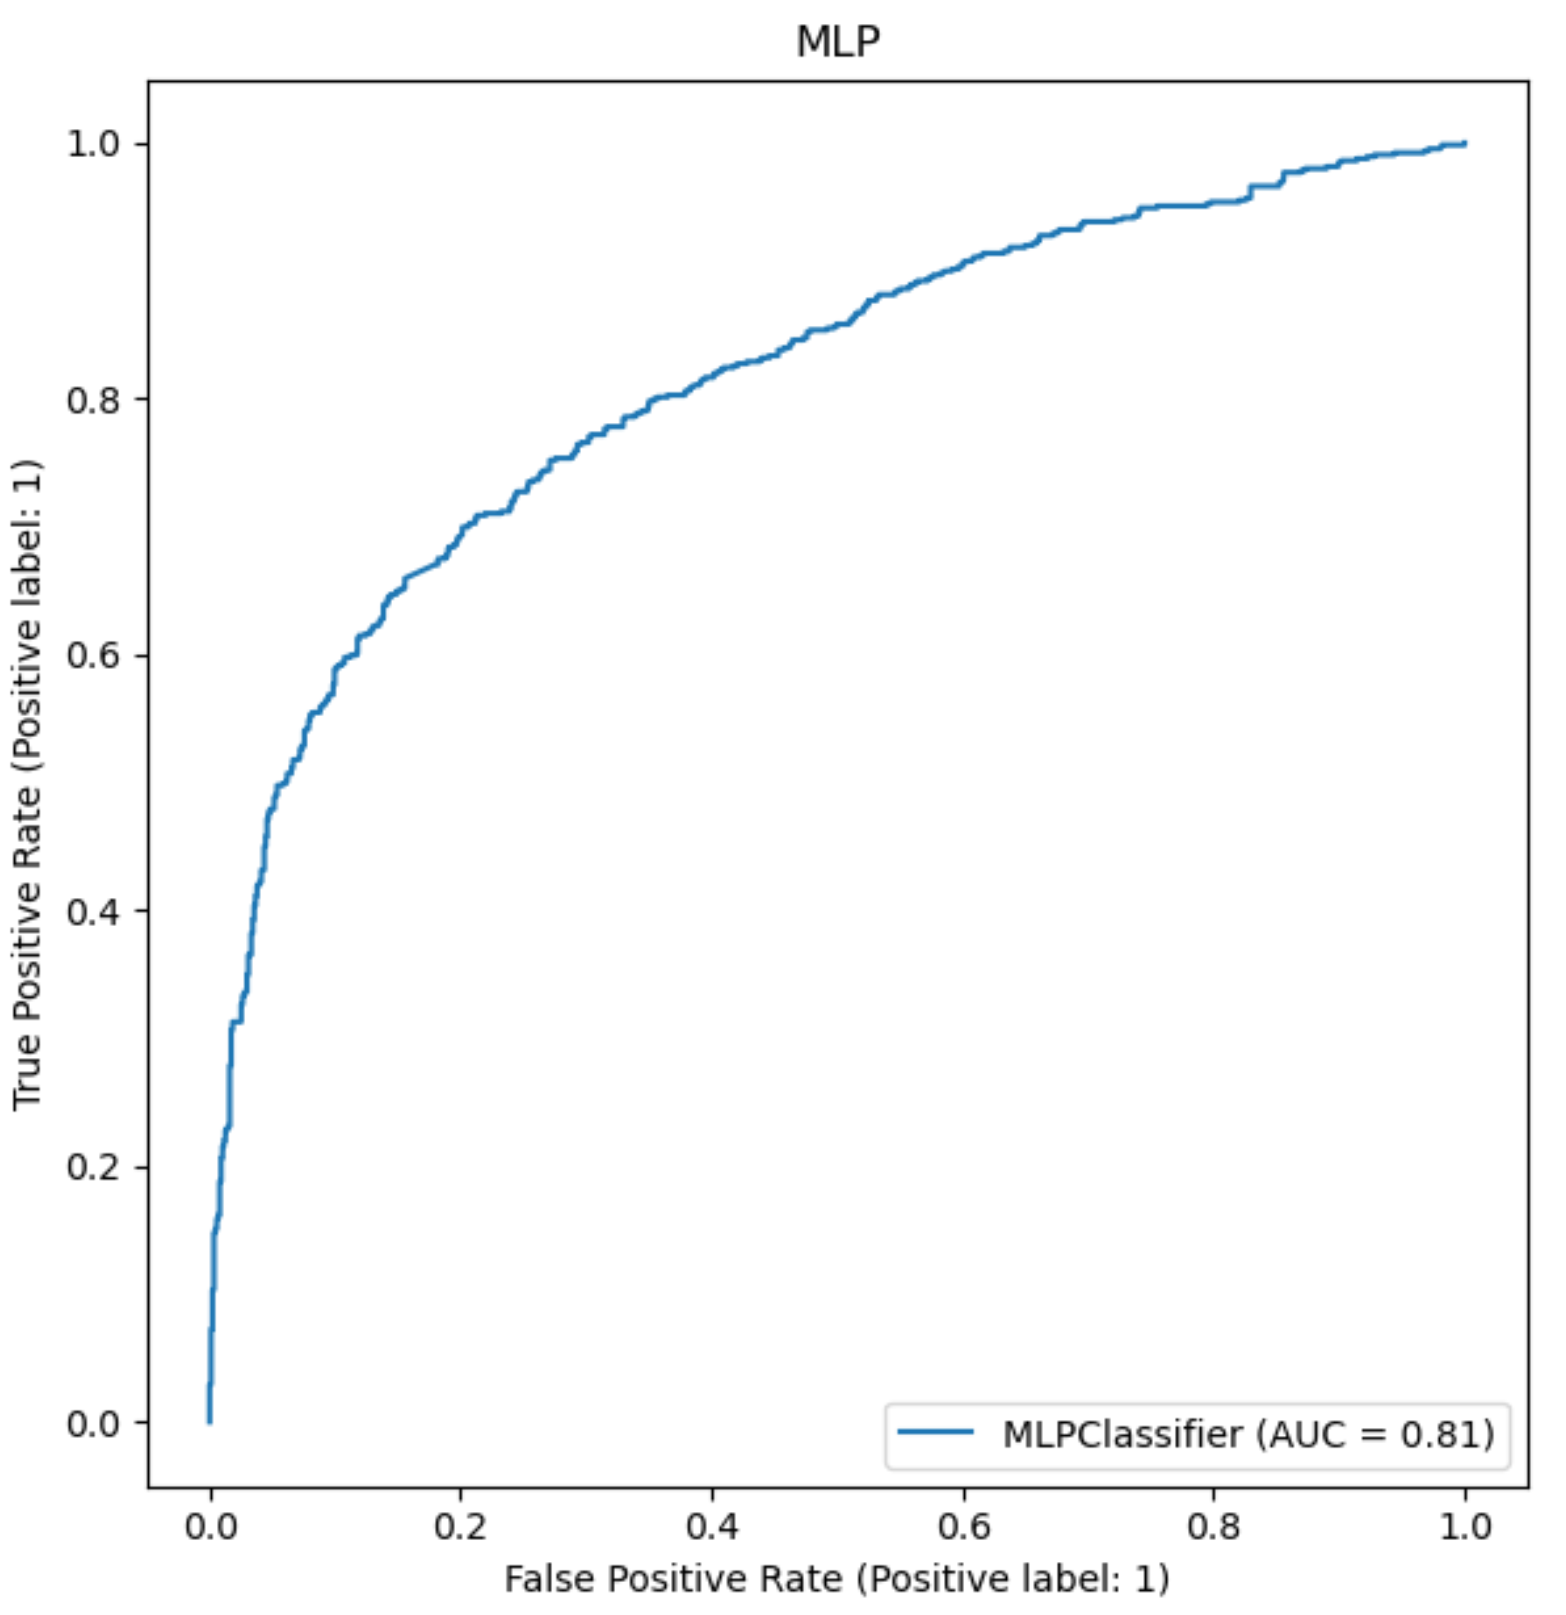
\includegraphics[width=\linewidth]{images/mlp_plot.png}
\end{minipage}\hfill
\begin{minipage}[b]{.45\linewidth}
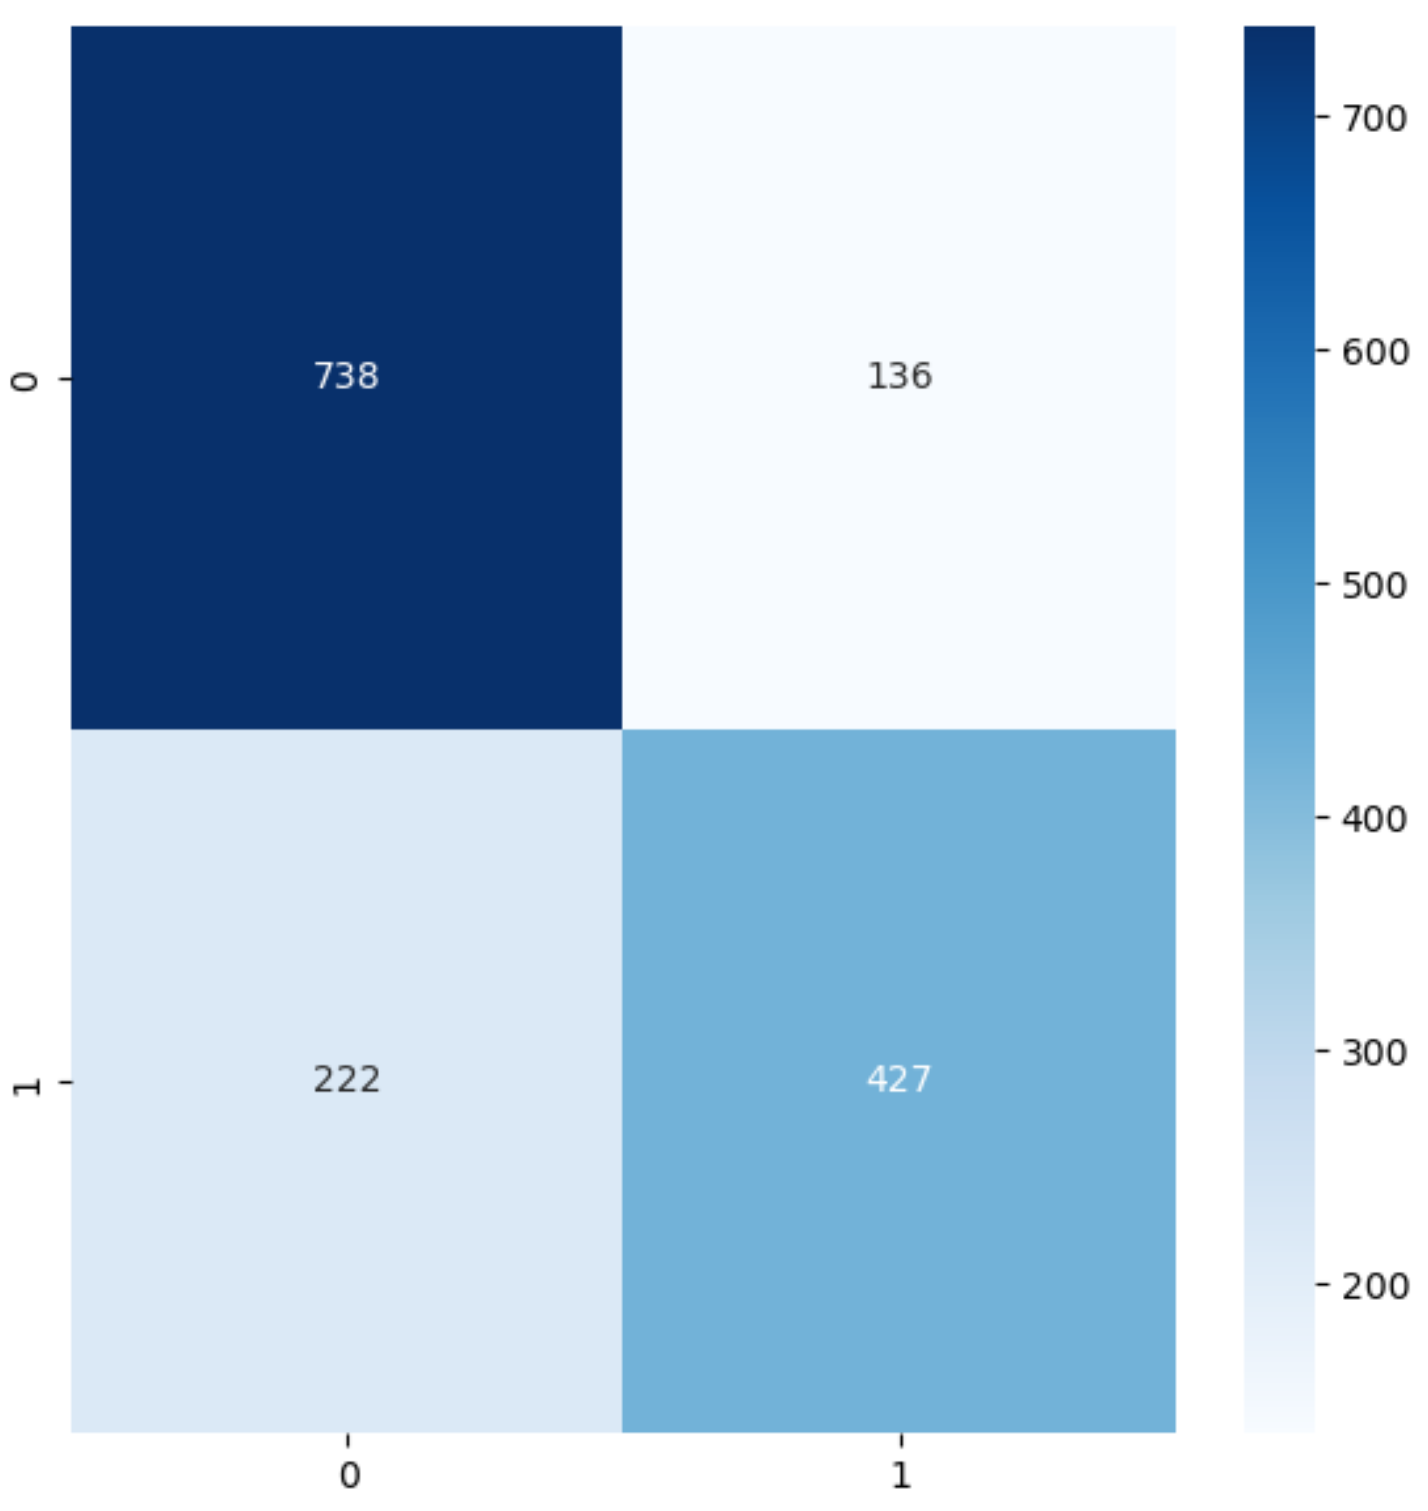
\includegraphics[width=\linewidth]{images/mlp_heatmap.png}
\end{minipage}\hfill

%------------------------------------------------

\section*{Conclusion}

To conclude, the application of Natural Language Processing (NLP) in machine learning has proven to be a powerful tool for classifying Twitter posts as pertaining to natural disasters or not. The results of our research project indicate that the multinomial naive Bayes model performed the best, with an accuracy rate of 80.21\% when classifying previously unseen and unclassified Twitter posts related to natural disasters. Our work is part of a Kaggle competition that highlights the potential of NLP and machine learning to address real-world problems, particularly in the context of emergency response during natural disasters.

This research has demonstrated the effectiveness of NLP and machine learning in the area of natural disaster response. As technology continues to evolve, there is a growing need for innovative solutions that can process large amounts of data quickly and accurately. Our project shows that NLP and machine learning can provide a promising avenue for addressing this challenge. We hope that this research will inspire others to continue exploring the potential of these technologies to develop new and innovative solutions for real-world problems.

%\begin{wrapfigure}{l}{0.42\textwidth} % Inline image example, use an 'r' column type to position the figure on the right
	%\includegraphics[width=\linewidth]{fish.png}
	%\caption{An example fish.}
%\end{wrapfigure}

%----------------------------------------------------------------------------------------
%	BIBLIOGRAPHY
%----------------------------------------------------------------------------------------

\bibliographystyle{unsrt}

\bibliography{sample.bib}

%----------------------------------------------------------------------------------------

\end{document}
